\documentclass[10pt,a4paper]{article}
\usepackage[a4paper,margin=1.8cm]{geometry}
\usepackage[T1]{fontenc}
\usepackage{lmodern}
\usepackage{microtype}
\usepackage{booktabs}
\usepackage{tabularx}
\usepackage{array}
\usepackage[table]{xcolor}
\usepackage{enumitem}
\usepackage{titlesec}
\usepackage{url}
\usepackage[colorlinks=true,linkcolor=blue!50!black,urlcolor=blue!50!black]{hyperref}
\usepackage{graphicx}
\setlength{\textfloatsep}{1.6ex plus 0.6ex}
\setlength{\floatsep}{1.4ex plus 0.6ex}
\renewcommand{\topfraction}{0.9}
\renewcommand{\textfraction}{0.08}
\renewcommand{\floatpagefraction}{0.85}
\newcommand{\figcap}[1]{\caption{\footnotesize #1}}
\setlist{nosep,leftmargin=1.3em}
\titlespacing*{\section}{0pt}{1.4ex}{0.6ex}
\setlength{\parindent}{0pt}
\setlength{\parskip}{0.55ex}
\renewcommand{\arraystretch}{1.12}
\newcommand{\iss}[1]{\href{https://github.com/JieGH/RVV_code_gen_via_MLIR_xDSL/issues/#1}{\##1}}
\newcommand{\good}[1]{\textcolor{green!45!black}{\textbf{#1}}}
\newcommand{\bad}[1]{\textcolor{red!70!black}{\textbf{#1}}}
\newcommand{\key}[1]{\textbf{\textcolor{blue!55!black}{#1}}}
\newcommand{\callout}[1]{\fcolorbox{blue!50!black}{blue!4}{\parbox{0.96\textwidth}{#1}}}
\titleformat{\section}{\large\bfseries}{\thesection}{0.6em}{}

\graphicspath{{issue-54-figs/simple/es/}}
\renewcommand{\figurename}{Figura}
\hyphenpenalty=2000
\emergencystretch=2em
\title{\vspace{-1.2cm}\textbf{Una columna cada vez}\\[2pt]\large La solución del issue \iss{54} en palabras sencillas: qué cambia en el código y por qué ayuda}
\author{RVV\_code\_gen\_via\_MLIR\_xDSL, \texttt{pure-xdsl}; SpacemiT X60 (RVV 1.0, VLEN 256)}
\date{29 de octubre de 2026. Guía corta; el informe completo es \texttt{issue-54-brief-es.pdf}. Versión en español}
\begin{document}
\maketitle\vspace{-1.5ex}

\callout{
\textbf{El problema.} Nuestro benchmark B3 cae a menudo en un \emph{estado lento}: unos 4,6 GOPs en lugar de 7,0. Lo provoca el empaquetador
de B, porque lee B con un patrón que el hardware de caché maneja mal.\\[3pt]
\textbf{La solución.} \key{Leer B una columna cada vez, 32 números por carga, y escribir esos números en su sitio de Bc.}\\[3pt]
\textbf{El resultado.} Nuestro diseño pasa de 4,63 a 7,03 GOPs, y el diseño de referencia de Adri\'an de 4,49 a 7,14 GOPs con la misma solución.
\key{Bc sale idéntico byte a byte, así que los resultados no pueden cambiar.}}

\section{Qué hace el empaquetador}
B se guarda columna a columna. Los números de una columna están seguidos en memoria; la columna siguiente empieza $K\times4$ bytes más allá
(\texttt{ldb*4} = 1536 B para $K=384$). El empaquetador copia B en un búfer llamado Bc, en el orden en que lo leerá el microkernel. Es solo una
copia: no hace ninguna operación aritmética.

\section{La forma actual y la solución}
\begin{figure}[!ht]
\centering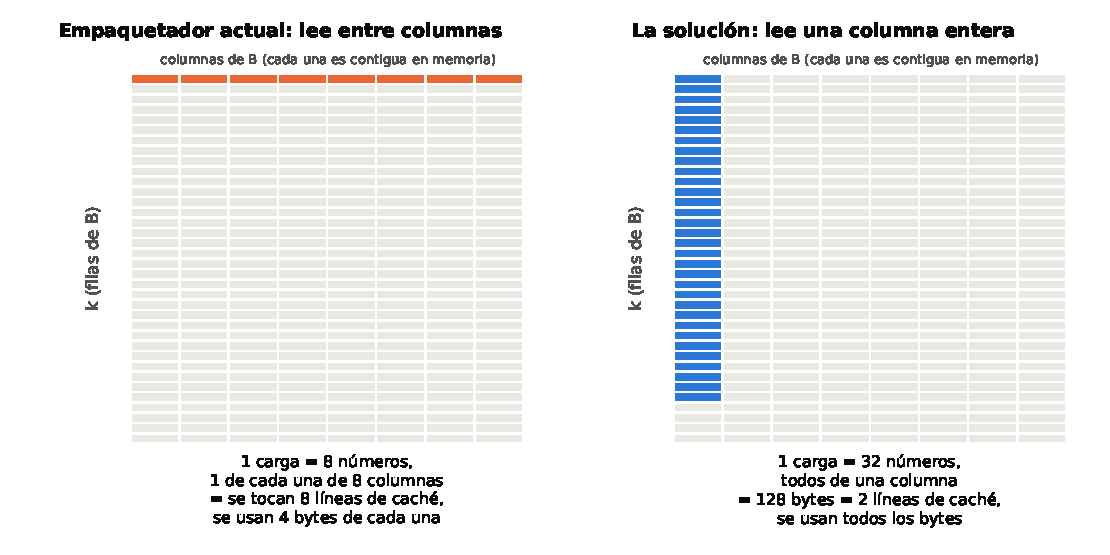
\includegraphics[width=0.8\textwidth]{fig_simple_read.pdf}
\figcap{B dibujada como 8 columnas de 36 valores (cada cuadrito es un número fp32). Los cuadritos de color son los números que lee una carga vectorial.}
\end{figure}
\begin{itemize}
\item \textbf{Empaquetador actual.} Cada carga toma 1 número de cada una de 8 columnas. \key{Eso toca 8 líneas de caché distintas y usa solo 4 bytes
  de cada línea de 64 bytes}, y la carga siguiente vuelve a empezar a 1536 B de la anterior. El precargador de L1D se vuelve entonces menos eficaz, y
  el empaquetado y el cálculo se hacen más lentos.
\item \textbf{La solución.} Cada carga toma 32 números de una columna. \key{Son 128 B seguidos: 2 líneas de caché, con todos los bytes usados}, y la carga
  siguiente continúa justo detrás. Es el orden de acceso para el que están hechos los precargadores.
\item \textbf{Adónde fue el salto.} El salto sigue siendo necesario, porque Bc está organizado por filas de $k$. Lo hemos pasado de la carga al
  \emph{almacenamiento}: las cargas de la matriz grande B van ahora en orden, y el almacenamiento con paso escribe en Bc.
\end{itemize}

\section{Qué cambia en las intrínsecas}
Solo cambian tres llamadas. \texttt{e32} significa elementos de 32 bits (fp32); \texttt{m1} y \texttt{m4} son el LMUL, cuántos registros vectoriales
usa una instrucción.
\begin{center}\footnotesize
\begin{tabular}{@{}p{1.6cm}p{4.7cm}p{5.2cm}p{4.4cm}@{}}
\toprule
 & empaquetador actual & la solución & qué significa \\
\midrule
longitud & \texttt{vsetvl\_e32m1} & \texttt{vsetvl\_e32m4} & hasta 8 números $\to$ hasta 32 \\
carga & \texttt{vlse32\_v\_f32m1(src, ldb*4, vl)} & \texttt{vle32\_v\_f32m4(src, vl)} & con paso entre columnas $\to$ simple, en orden \\
almacén. & \texttt{vse32\_v\_f32m1(dst, v, vl)} & \texttt{vsse32\_v\_f32m4(dst, RR*4, v, vl)} & 8 juntos $\to$ uno por fila de Bc \\
\bottomrule
\end{tabular}
\end{center}
El mismo código de la solución, tal como está en \texttt{pack\_CB} del diseño de referencia (se omite el \texttt{if} que protege la ruta vectorial), y las
instrucciones RISC-V en que se convierte:
{\footnotesize\begin{verbatim}
size_t vl = __riscv_vsetvl_e32m4((size_t) len);              // len es como mucho 32
vfloat32m4_t v = __riscv_vle32_v_f32m4(src, vl);             // 32 números de una columna de B
__riscv_vsse32_v_f32m4(dst, (ptrdiff_t) RR * 4, v, vl);      // un número por fila de Bc

actual:    vsetvli zero,a7,e32,m1,ta,ma
           vlse32.v v24,(a4),t1  (t1 = 1536 B)
solución:  vsetvli t4,t4,e32,m4,ta,ma
           vle32.v  v24,(a3)
           vsse32.v v24,(s6),a5  (a5 = RR*4)
\end{verbatim}}
\begin{figure}[!ht]
\centering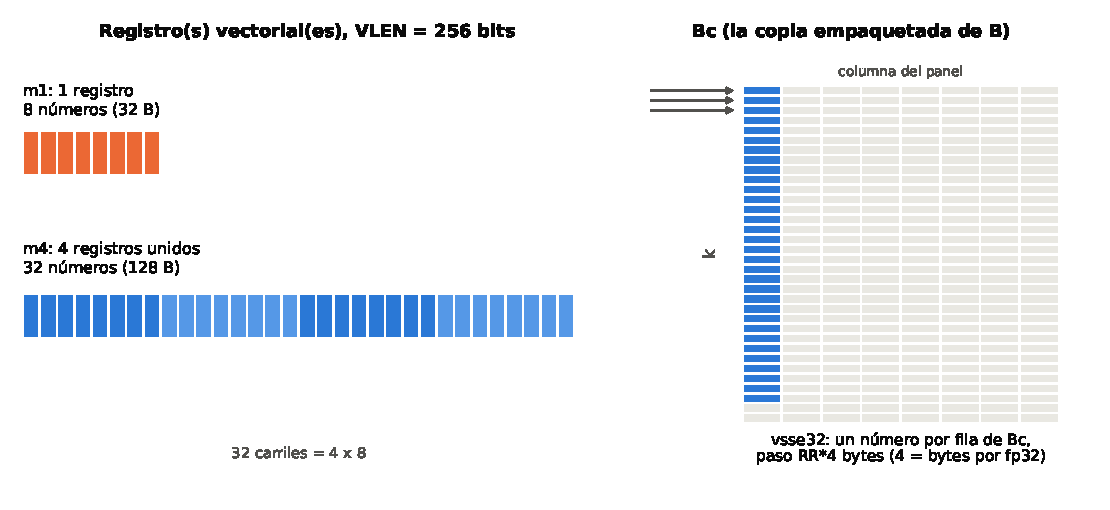
\includegraphics[width=0.9\textwidth]{fig_simple_lmul_store.pdf}
\figcap{Izquierda: un registro \texttt{m1} guarda 8 números; \texttt{m4} une 4 registros y guarda 32. Derecha: los 32 números de una columna de B
van a una columna de Bc, un número por fila.}
\end{figure}

\callout{\textbf{Dos 4 distintos.} En \texttt{ldb*4} y \texttt{RR*4}, el 4 son los \emph{bytes de un número fp32}, porque las intrínsecas toman los
pasos en bytes. En \texttt{m4}, el 4 es \emph{cuántos registros se unen}: $4\times8=32$ números.}

\section{Por qué el resultado no puede cambiar}
Un empaquetador solo copia. Las dos versiones ponen cada número de B en el mismo sitio de Bc, \texttt{Bc[p*NR*kc + k*NR + j]}; solo cambia el orden de la
copia. Lo comprobamos byte a byte en el equipo anfitrión para el empaquetador parcheado del diseño de referencia (1008 casos), y el microkernel, el
bloqueo y la organización de Bc no se tocan.

\section{Resultado}
\begin{figure}[!ht]
\centering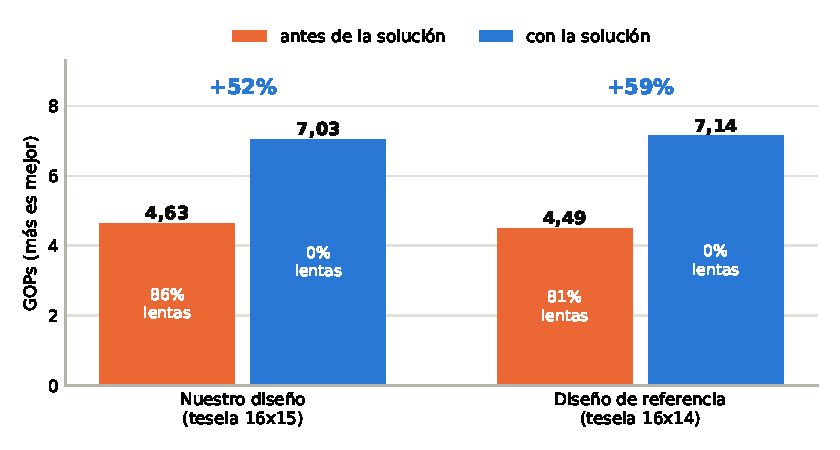
\includegraphics[width=0.62\textwidth]{fig_simple_result.pdf}
\figcap{B3 (64$\times$384$\times$384), compilación sin instrumentar, protocolo de referencia, núcleo 4. Nuestro diseño: serie 1, 22 de octubre. Diseño de
referencia: 29 de octubre, 3 lanzamientos (4,39--4,60 $\to$ 7,11--7,18). Texto en las barras: porcentaje de repeticiones lentas.}
\end{figure}
\key{La solución elimina el estado lento en los dos diseños}: el 86\% y el 81\% de repeticiones lentas pasan a 0\%.

\section{\textquestiondown Merece la pena?}
Una opción más simple es el empaquetador escalar que el generador ya tiene (\texttt{use\_scalar\_pack}). Ayuda, pero no es seguro en todas partes:
38\% de repeticiones lentas en B3 con la tesela por defecto, 4,64 GOPs en B3\_K256 con 16$\times$15, y 3--4\% menos en B2. \key{La solución es la mejor, o está
a menos del 1\% de la mejor, en 11 de 12 celdas.} Lo que aún no sabemos es cuánto del tiempo de un modelo real se pasa en capas con M pequeña y K grande como B3;
eso decide cuánto vale la solución en conjunto.

\section{Preguntas probables}
\textbf{\textquestiondown Por qué no transponer B antes?} Una transposición es una copia extra de toda la matriz, y después aún hay que construir Bc. \key{La solución
hace la transposición dentro del propio empaquetado, en la misma pasada}: sin copia extra, y el GEMM se llama como antes.

\textbf{\textquestiondown Cambia el resultado leer en otro orden?} No. Un empaquetador solo copia, y cada número cae en la misma dirección de Bc que antes
(Bc es idéntico byte a byte). Solo cambia el orden de la copia.

\textbf{\textquestiondown Hace más lento el empaquetado?} Un poco, en una repetición rápida: la media solo del empaquetado con 16$\times$15 en B3 es 0,8218 ms frente a 0,6443 ms
del empaquetador vectorial actual. Pero \key{nunca pasa a lento}, mientras que el actual pasa el 91\% de sus repeticiones a 1,1994 ms. Además necesita menos
instrucciones: 60 cargas por panel en lugar de 256 (B3, tesela por defecto).

\textbf{\textquestiondown Por qué ocurre en B3 y no en todas partes?} No está del todo explicado. Influye el paso entre las 8 columnas (1536 B con $K=384$), y el relleno de
\texttt{ldb} cambia el estado, pero sin un patrón simple (\iss{49}). Las teselas más pequeñas lo evitan en algunas celdas (B3 con 16$\times$6) y en otras no
(B3 con 16$\times$8: 3,83 GOPs).

\textbf{\textquestiondown Es solo mi diseño, o también el de referencia?} Los dos. La referencia empaqueta B en el mismo orden, un número por carga con el mismo paso de
1536 B, y en B3 con 16$\times$14 estuvo lenta el 81\% de las repeticiones (4,49 GOPs). El desarrollador de la referencia no ve ningún fallo en el código de empaquetado en sí, lo cual encaja:
el resultado es correcto, y solo sufre la velocidad.

\textbf{\textquestiondown Empeoró mi empaquetador vectorial el problema?} En la mayoría de las celdas, sí. Con la tesela por defecto está lento el 86\%, frente al 38\% del empaquetador escalar.
Volver al escalar tampoco elimina el estado lento.

\textbf{\textquestiondown Por qué \texttt{m4} y no \texttt{m1}?} La versión \texttt{m1} de la misma idea (\texttt{col-g1}) tampoco es lenta nunca. Se eligió \texttt{m4}
porque así una carga cubre 2 líneas de caché enteras y hacen falta menos instrucciones. Un empaquetador solo copia, así que usar 4 de los 32 registros
por grupo no cuesta nada.

\textbf{\textquestiondown Bastaría una tesela más pequeña, o rellenar la matriz?} No de forma fiable, como arriba: las dos cosas cambian el estado sin patrón simple, mientras que la
solución no dio ninguna repetición lenta en ninguna de las 18 celdas que ejecutamos.

\textbf{\textquestiondown Hasta dónde llegan los números de la referencia?} Solo B3, con dos teselas. Con 16$\times$14 pasó de 4,49 a 7,14 GOPs; con 16$\times$16 de 4,20 a
4,41, una mejora mucho menor, así que allí quedan otros efectos. Nuestro diseño se ejecutó en 18 celdas GEMM.

\textbf{\textquestiondown Cambiaste el repositorio de Adri\'an?} No. La solución se aplica a una copia preparada de \texttt{gemm\_blis.c} con \texttt{ref\_pack\_fix.py};
los archivos de \texttt{ext/} no se tocan.
\end{document}
